\section{Evaluation}
Our evaluation would take the form of a case study in which we compare different approaches to testing the {\tt function checkRows()} in Sample Code \ref{dom0}, and measure how much coverage each approach can achieve.
Existing approaches to concolic testing JavaScript~\cite{kudzu, jalangi} focus on generating input parameters.  
Yet the {\tt function checkRows()} does not take any input arguments.  Thus these approaches would likely execute the function by simply calling {\tt checkRows()}.
Therefore, in this case study we will call the {\tt function checkRows()} in the following 3 scenarios and measure how much code is covered in each case.  
\begin{compactitem}
\item {\em Without HTML}
\item {\em Existing HTML} from the application
\item \tool generated HTML
\end{compactitem}

For each approach, we would follow the same methodology of loading and execution the function:
\begin{compactitem}
\item Open the target URL in the Web browser
\item Load the HTML (except {\em Without HTML})
\item Execute the target code
\item Measure coverage
\end{compactitem}
Recalling from the Implementation section, the 4 steps above are identical to the initial 4 steps that our concolic driver would take in each iteration.  Additionally the concolic driver would take the executed paths as feedback and generate new HTML.  
For {\tt function checkRows()}, we can simply call the function via {\tt checkRows()} because it does not take any input arguments.

\begin{figure}
\centerline{\scalebox{0.38}{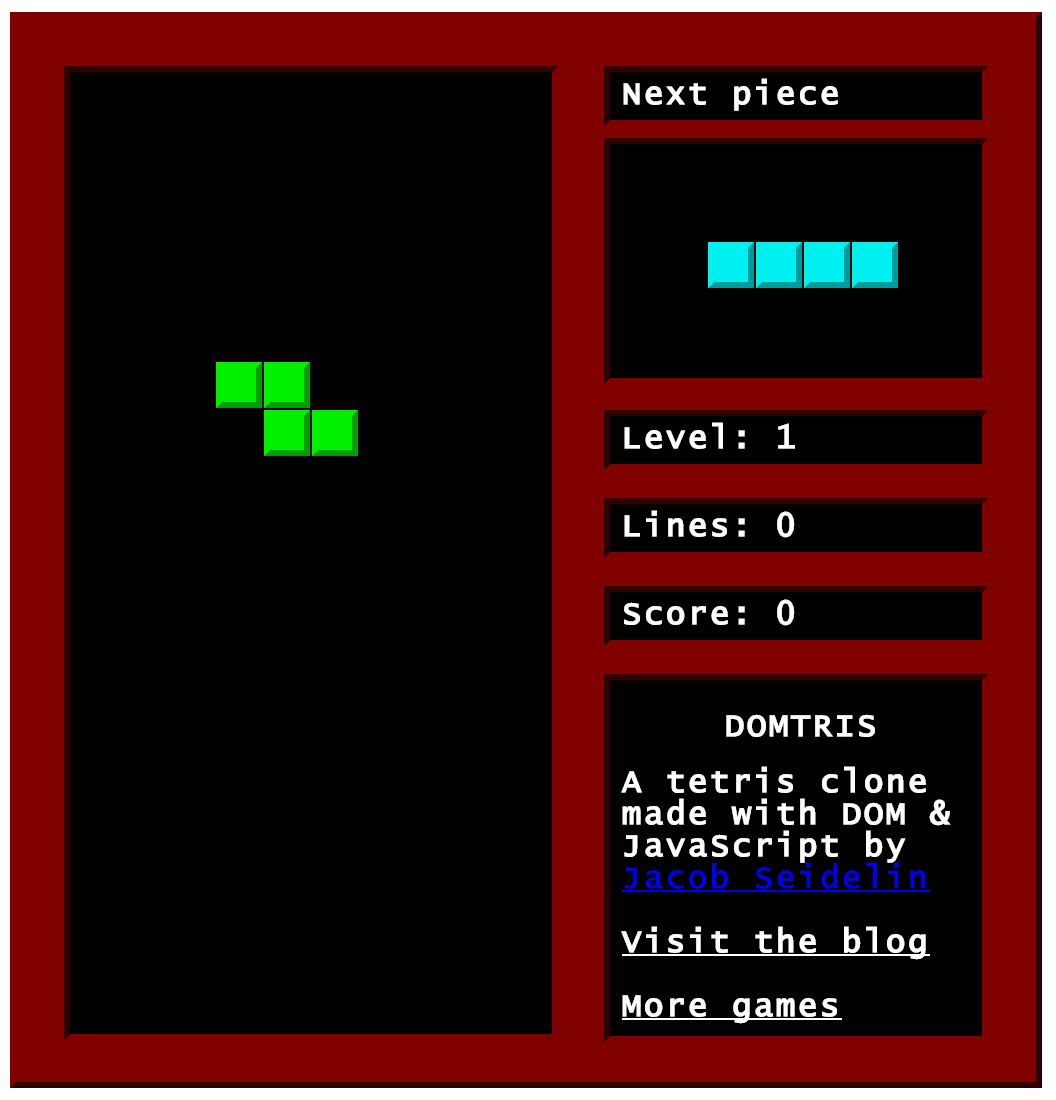
\includegraphics[natwidth=1056,natheight=1100]{domtris.png}}}
\caption[DOMtris game field]{The DOMtris game field has 20 rows, thus {\tt field.children.length} is set to be 20 in our evaluation.}
\label{domtrisfield}
\end{figure}

\begin{figure}[h]
\centerline{
\begin{tabular}{*2l|*3c}
\hline
& & \multicolumn{3}{c}{Count (Number Of)} \\ 
App & Function & Statements & Branches & Paths \\ \hline
DOMtris & checkRows() & 6 & 4 & 41 \\ \hline
\end{tabular}
}
\caption{Number of Statements, Branches and Paths of function being evaluated.}
\label{paths}
\end{figure}
%\slopypar{


%}

\header{Counting Execution Paths.}
Figure \ref{paths} shows the number of statements, branches and paths that the function has.   
When counting the number of paths in the {\tt function checkRows()} in Sample Code \ref{dom0}, 
the original code does not pose an upper bound to the number of times the {\tt for} loop would get iterated because {\tt field.children.length} can be any value.
Therefore, we would set {\tt field.children.length} to a specific number for calculating the total number of possible execution paths in the function.
{\tt field} is set to have 20 children because the actual application always has 20 rows (Figure \ref{domtrisfield}). 
The following shows how the number of statements, branches and paths are counted for the {\tt function checkRows()}:
\begin{compactitem}
\item {\em Statements}: 6, {\tt line 2} to {\tt line 7}, inclusive.
\item {\em Branches}: 2 + 2. The {\tt for} loop has 2 branches: {\tt stay} and {\tt break}; plus the {\tt if} condition also has 2 branches: {\tt true} and {\tt false}. 
\item {\em Paths}: 20 ({\tt stay} branch in for loop) * 2 ({\tt true} and {\tt false} branches in {\tt if} statement) + 1 ({\tt break} branch).
\end{compactitem}

\begin{figure}[h]
\centerline{
\begin{tabular}{l|*3c}
\hline
& \multicolumn{3}{c}{Count (Number Of)} \\	
Approach & Statements & Branches & Paths \\ \hline
Optimal & 6 & 4 & 41 \\ \hline
{\em Without HTML} & 1 & 0 & 0 \\ 
{\em Existing HTML} & 5 & 3 & 1 \\ 
\tool & 6 & 4 & 41 \\ \hline
\end{tabular}
}
\caption{Statement, Branch and Path coverage of different approaches to testing the {\tt function checkRows()}. The Optimal approach is stated here to reference what perfect coverage would look like.}
\label{coverage}
\end{figure}

\header{Coverage Results.}
Figure \ref{coverage} shows the coverage results of different approaches to testing the {\tt function checkRows()}.  

The {\em Without HTML} approach cannot cover any statement because the first statement in the {\tt function checkRows()} is already a DOM operation requiring the existence of an element with ID {\tt "field"}.

The {\em Existing HTML} approach is able to cover 5 statements inclusively from {\tt line 2} to {\tt line 6} because the original HTML already has 20 rows inside {\tt field}.  
However the {\em Existing HTML} approach cannot cover the statement in {\tt line 7} because the rows do not have any children at the start of the game. 
{\em Existing HTML} is able to cover 3 of the 4 possible branches: both the {\tt stay} and {\tt break} branches in the {\tt for} loop, and the {\tt false} branch in the {\tt if} condition. 
Yet, the {\em Existing HTML} approach is able to cover only one path because going through a different path in {\tt function checkRows()} requires another unique DOM tree structure.  

\tool is able to cover all possible paths in {\tt function checkRows()} because we have set {\tt field.children.length} to be 20, 
and all the conditions (the {\tt for} loop and the {\tt if} condition) inside the function are all driven by DOM operations.  
In case when there are conditions that are driven by other data types, our solver would have to be extended to support these data types.    

\header{Discussion.}
In the specific example of {\tt function checkRows()}, using only the existing HTML is sufficient to achieve high statement coverage (5/6 or 83\%) and high branch coverage (3/4 or 75\%).  

Concolic testing often takes additional time, in our small example the DOM solver would take about 15 to 30 seconds to generate each additional HTML on a MacBook pro with a 2.0GHz quad core Intel i7 processor and 16GB RAM.
Thus whether concolic testing is worth it would depend on how much additional coverage the concolic approach would provide, and the benefits of having the additional coverage.  

While \tool covers only 1 additional statement ({\tt line 7}) and only 1 additional branch ({\tt true} branch of the {\tt if} condition) compared to {\em Existing HTML}, 
the additionally covered statement is responsible for updating the game's score, and scoring is a core functionality of DOMtris.  
Another benefit of \tool is that it covers all the different paths that generate the different permutations of increasing the score.  

Our current concolic driver is primitive in the sense that it exhaustively tries to cover all execution paths possible.  
In the future, it may be worth investigating if it is possible to design a smarter concolic driver that can give priority to execution paths that would yield the highest marginal benefit of additional coverage: 
e.g. highest additional branch coverage, the most diverse permutation of increasing the score, etc.  
That way the tester can exercise concolic testing partially, combine concolic testing with other less expensive testing methods (e.g. ~\cite{feedbackConcolic, hybridconcolic}), and still achieve certain desired outcomes without incurring the full costs associated with complete concolic execution.  
Thus having a prioritized concolic engine would give the tester greater control to manage the costs and benefits of the testing life cycle.  

% yahoo
% Tinysort
%  http://tinysort.sjeiti.com/
% Zen Coding
%  http://zen.sjeiti.com/
% DOMtris
%  http://www.ugrad.cs.ubc.ca/~k5r4/nbpAFZyrx5o/tracing/domtris/domtris.html
% Tudu
%  http://app.rasc.ch/tudu/welcome.action
% Knockout:
%  http://knockoutjs.com/examples/ 
% JQuery Widget: 
%  http://jqueryui.com/demos/
%  http://wijmo.com/widgets/
% Tizen
%   https://developer.tizen.org/downloads/sample-web-applications
%			mancala
